\documentclass{beamer}

\makeatletter
\def\input@path{{Padova/}}
\makeatother

\usetheme{Padova}

\graphicspath{ {images/} }

\title{Migliorare la Business Intelligence con l'AI}
\subtitle{Discussione di Laurea Triennale in Informatica}
\author{Riccardo Stefani}
\date{23 Luglio 2025}


\begin{document}

	\maketitle

	\begin{frame}{Indice}
		\tableofcontents
	\end{frame}


	\section{Introduzione}

	\begin{frame}{Introduzione - Oribea}
		Lorem ipsum dolor sit amet, consectetur adipiscing elit. Sed do eiusmod tempor incididunt ut labore et dolore magna aliqua.

		\begin{itemize}
			\item Ut enim ad minim veniam, quis nostrud exercitation
			\item Duis aute irure dolor in reprehenderit in voluptate
			\item Excepteur sint occaecat cupidatat non proident
		\end{itemize}

		\begin{figure}[h]
			\centering
			
\includegraphics[width=0.5\textwidth]{oribea-logo.png}
		\end{figure}
	\end{frame}

	\begin{frame}{Introduzione - Il progetto}
		Sed ut perspiciatis unde omnis iste natus error sit voluptatem accusantium doloremque laudantium.

		\begin{block}{Obiettivi del progetto}
			Totam rem aperiam, eaque ipsa quae ab illo inventore veritatis et quasi architecto beatae vitae dicta sunt explicabo.
		\end{block}
	\end{frame}


	\section{Analisi delle vendite}

	\begin{frame}{Analisi delle vendite - L'idea}
		\begin{columns}
			\begin{column}{0.6\textwidth}
				Nemo enim ipsam voluptatem quia voluptas sit aspernatur aut odit aut fugit, sed quia consequuntur magni dolores eos qui ratione voluptatem sequi nesciunt.

				\begin{itemize}
					\item Neque porro quisquam est, qui dolorem ipsum quia dolor sit amet
					\item Consectetur, adipisci velit, sed quia non numquam eius modi tempora
					\item Incidunt ut labore et dolore magnam aliquam quaerat voluptatem
				\end{itemize}
			\end{column}
			\begin{column}{0.4\textwidth}
				\begin{figure}
					\centering
					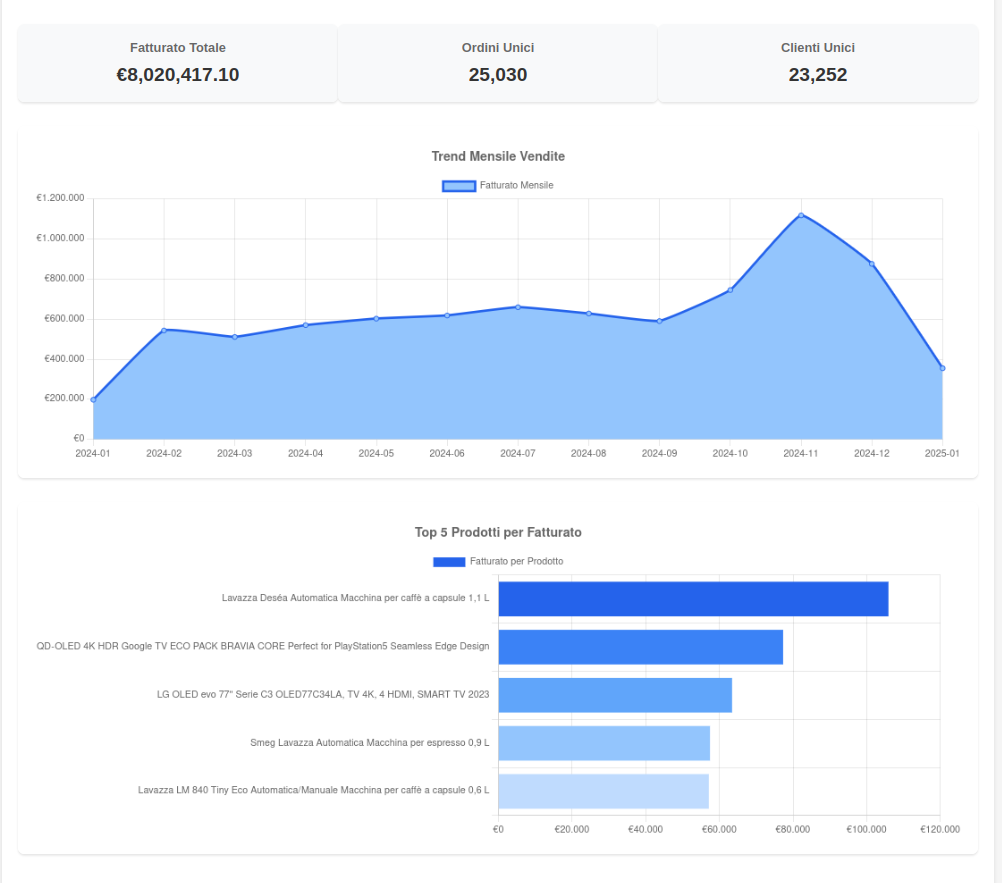
\includegraphics[width=\textwidth]{Oribea - Esempio di report delle vendite.png}
				\end{figure}
			\end{column}
		\end{columns}
	\end{frame}

	\begin{frame}{Analisi delle vendite - Preprocessing, Language processing, statistiche e grafici}
		Ut enim ad minima veniam, quis nostrum exercitationem ullam corporis suscipit laboriosam, nisi ut aliquid ex ea commodi consequatur.

		\begin{columns}
			\begin{column}{0.5\textwidth}
				\begin{block}{Preprocessing}
					Quis autem vel eum iure reprehenderit qui in ea voluptate velit esse quam nihil molestiae consequatur.
				\end{block}
			\end{column}
			\begin{column}{0.5\textwidth}
				\begin{block}{Language Processing}
					Vel illum qui dolorem eum fugiat quo voluptas nulla pariatur.
				\end{block}
			\end{column}
		\end{columns}
	\end{frame}

	\begin{frame}{Analisi delle vendite: Generazione PDF e HTML, invio di email}
		At vero eos et accusamus et iusto odio dignissimos ducimus qui blanditiis praesentium voluptatum deleniti atque corrupti quos dolores et quas molestias excepturi sint occaecati cupiditate non provident.

		\begin{alertblock}{Automazione}
			Similique sunt in culpa qui officia deserunt mollitia animi, id est laborum et dolorum fuga.
		\end{alertblock}
	\end{frame}


	\section{Sistema di raccomandazione}

	\begin{frame}{Sistema di raccomandazione - L'idea}
		Et harum quidem rerum facilis est et expedita distinctio. Nam libero tempore, cum soluta nobis est eligendi optio cumque nihil impedit quo minus id quod maxime placeat facere possimus.

		\begin{itemize}
			\item Omnis voluptas assumenda est, omnis dolor repellendus
			\item Temporibus autem quibusdam et aut officiis debitis aut rerum necessitatibus
			\item Saepe eveniet ut et voluptates repudiandae sint et molestiae non recusandae
		\end{itemize}
	\end{frame}

	\begin{frame}{Sistema di raccomandazione - Collaborative Filtering}
		Itaque earum rerum hic tenetur a sapiente delectus, ut aut reiciendis voluptatibus maiores alias consequatur aut perferendis doloribus asperiores repellat.

		\begin{block}{Algoritmo}
			$$ R_{u,i} = \frac{\sum_{v \in N(u)} sim(u,v) \cdot R_{v,i}}{\sum_{v \in N(u)} |sim(u,v)|} $$
		\end{block}
	\end{frame}

	\begin{frame}{Sistema di raccomandazione - Similarità}
		Hic tenetur a sapiente delectus, ut aut reiciendis voluptatibus maiores alias consequatur aut perferendis doloribus asperiores repellat.

		\begin{columns}
			\begin{column}{0.6\textwidth}
				\begin{itemize}
					\item Cosine Similarity
					\item Pearson Correlation
					\item Jaccard Similarity
				\end{itemize}
			\end{column}
			\begin{column}{0.4\textwidth}
				\begin{exampleblock}{Formula}
					$$ sim(u,v) = \frac{\sum_{i} R_{u,i} \cdot R_{v,i}}{\sqrt{\sum_{i} R_{u,i}^2} \cdot \sqrt{\sum_{i} R_{v,i}^2}} $$
				\end{exampleblock}
			\end{column}
		\end{columns}
	\end{frame}


	\begin{frame}{Sistema di raccomandazione - Formato di archiviazione delle matrici}
			\begin{columns}
				\begin{column}{0.6\textwidth}
					Nam libero tempore, cum soluta nobis est eligendi optio cumque nihil impedit quo minus id quod maxime placeat facere possimus.

					\begin{block}{Struttura dati}
						\begin{itemize}
							\item Matrici sparse per efficienza
							\item Compressione dei dati
							\item Indici per accesso rapido
						\end{itemize}
					\end{block}
				\end{column}
				\begin{column}{0.4\textwidth}
					\begin{figure}
						\centering
						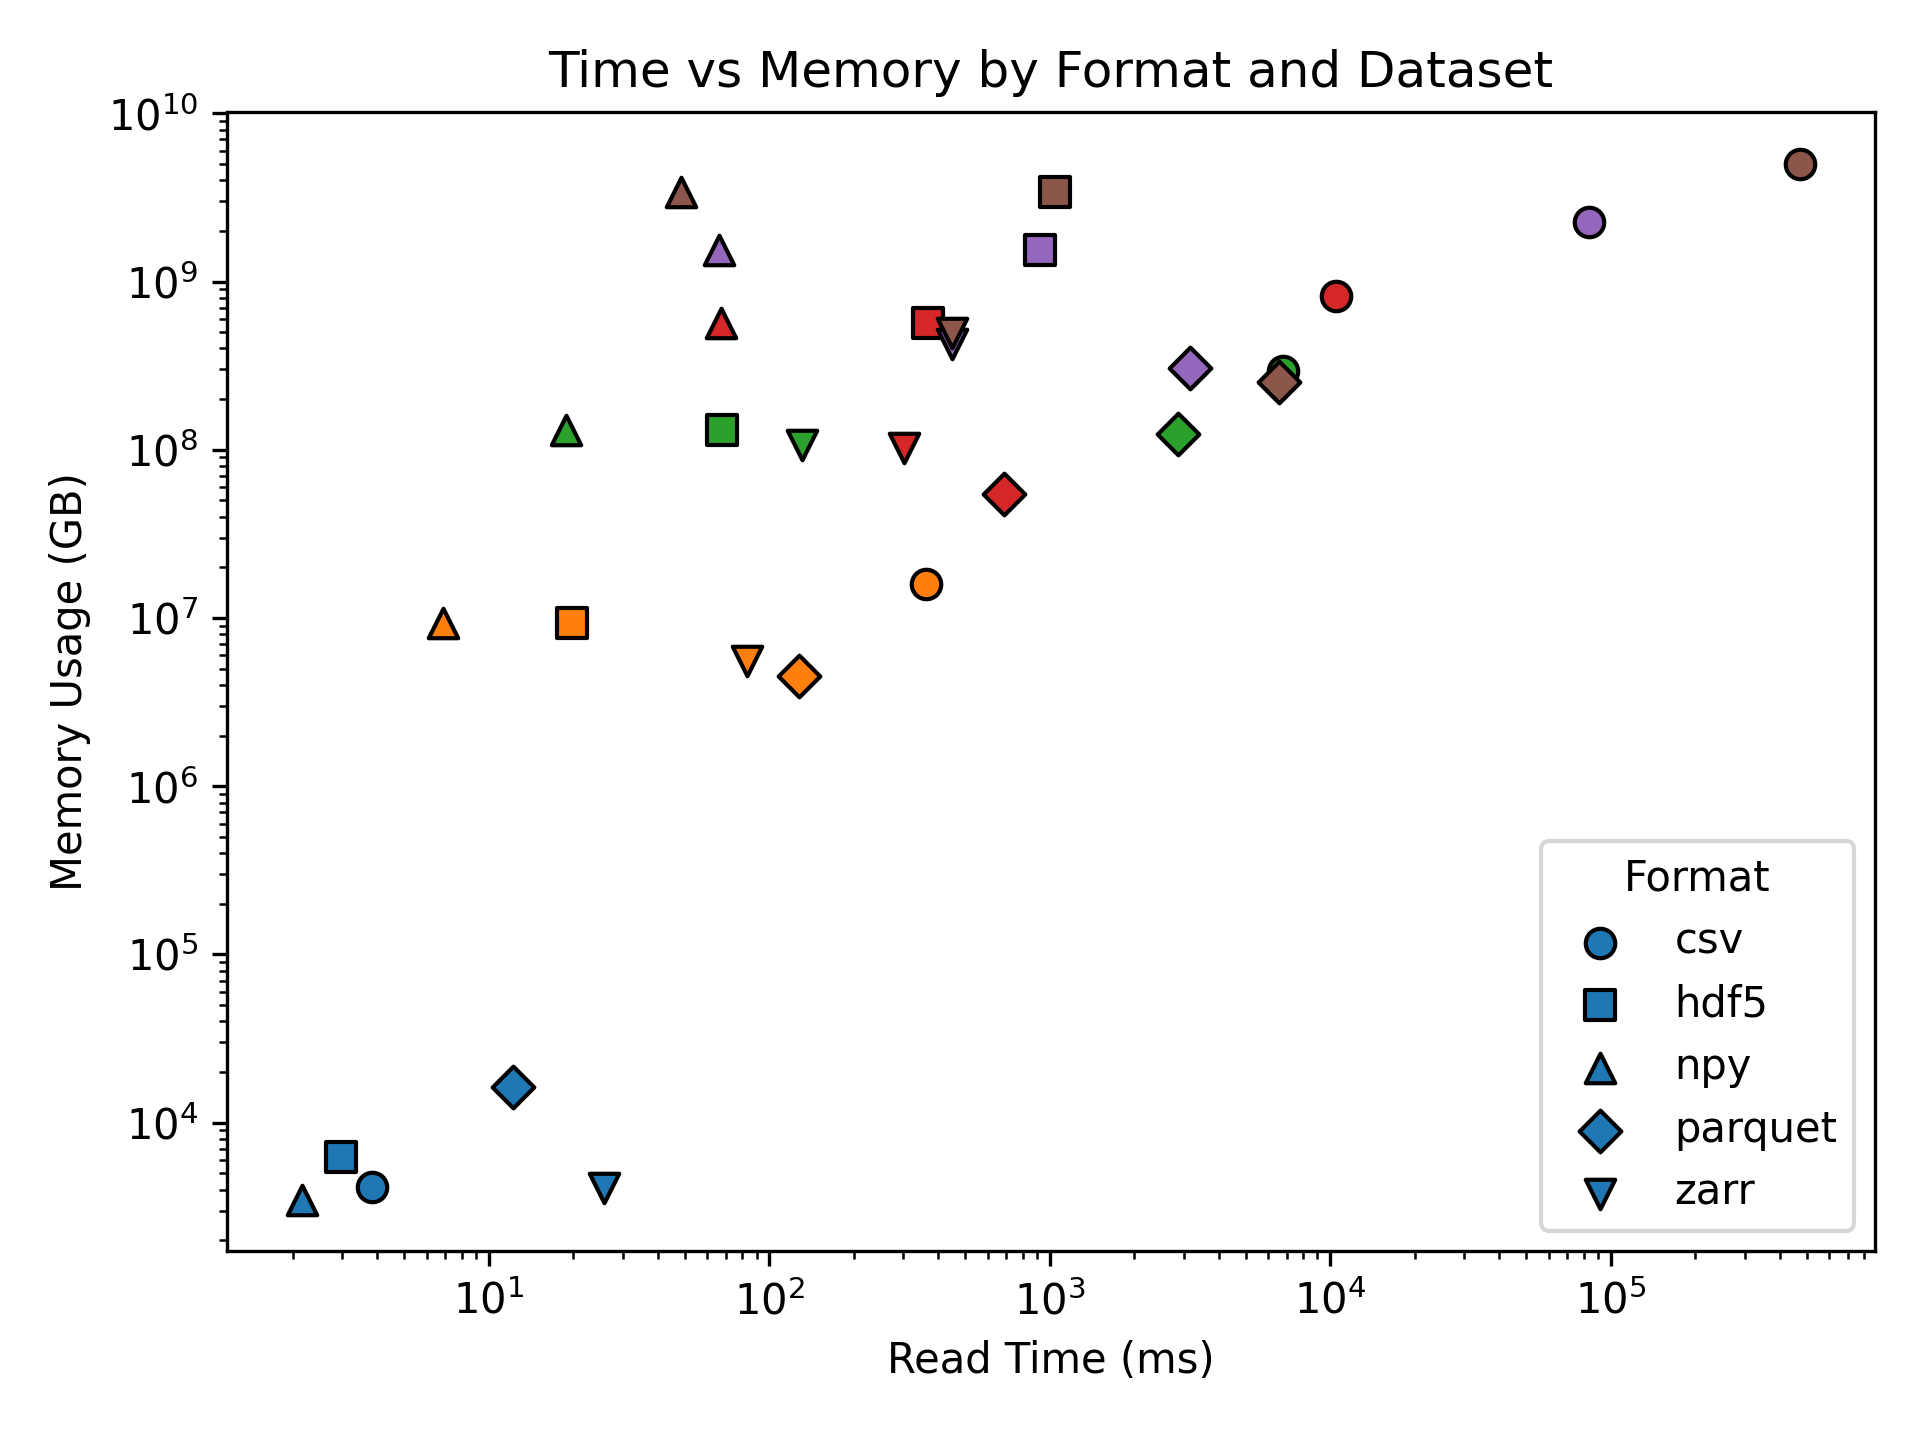
\includegraphics[width=\textwidth]{time_vs_memory.png}
					\end{figure}
				\end{column}
			\end{columns}
	\end{frame}

	\begin{frame}{Sistema di raccomandazione - Rank Fusion}
		Omnis voluptas assumenda est, omnis dolor repellendus. Temporibus autem quibusdam et aut officiis debitis aut rerum necessitatibus.

		\begin{alertblock}{Metodo di fusione}
			$$ Score_{final} = \alpha \cdot Score_{CF} + \beta \cdot Score_{content} + \gamma \cdot Score_{hybrid} $$
		\end{alertblock}
	\end{frame}

	\begin{frame}{Sistema di raccomandazione - Metriche di valutazione}
		Saepe eveniet ut et voluptates repudiandae sint et molestiae non recusandae.

		\begin{columns}
			\begin{column}{0.5\textwidth}
				\begin{block}{Precisione}
					$$ Precision@k = \frac{|R_k \cap T|}{k} $$
				\end{block}
			\end{column}
			\begin{column}{0.5\textwidth}
				\begin{block}{Recall}
					$$ Recall@k = \frac{|R_k \cap T|}{|T|} $$
				\end{block}
			\end{column}
		\end{columns}
	\end{frame}

	\begin{frame}{Sistema di raccomandazione - Explainability}
		Itaque earum rerum hic tenetur a sapiente delectus, ut aut reiciendis voluptatibus maiores alias consequatur.

		\begin{itemize}
			\item Interpretabilità delle raccomandazioni
			\item Trasparenza degli algoritmi
			\item Giustificazione delle scelte
		\end{itemize}
	\end{frame}


	\section{Deploy e frontend}

	\begin{frame}{Deploy e frontend - Integrazione con Google Cloud}
		Aut perferendis doloribus asperiores repellat. Hic tenetur a sapiente delectus.

		\begin{block}{Servizi utilizzati}
			\begin{itemize}
				\item Google Cloud Functions
				\item Cloud Storage
				\item Cloud SQL
				\item Cloud Scheduler
			\end{itemize}
		\end{block}
	\end{frame}

	\begin{frame}{Deploy e frontend - Interfacce frontend}
		Ut aut reiciendis voluptatibus maiores alias consequatur aut perferendis doloribus asperiores repellat.

		\begin{columns}
			\begin{column}{0.5\textwidth}
				\begin{block}{Dashboard}
					Interfaccia per la visualizzazione dei dati e delle statistiche
				\end{block}
			\end{column}
			\begin{column}{0.5\textwidth}
				\begin{block}{API}
					Endpoint REST per l'integrazione con sistemi esterni
				\end{block}
			\end{column}
		\end{columns}

		\begin{figure}
			\centering
			\begin{minipage}{0.4\textwidth}
				\centering
				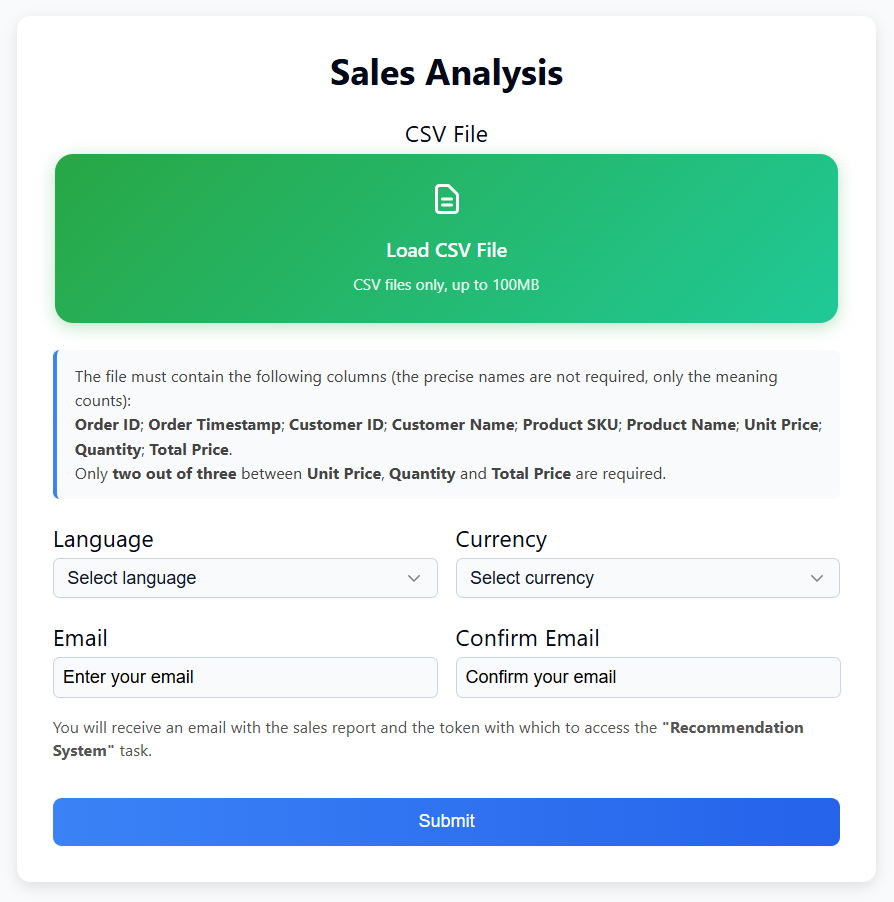
\includegraphics[width=\textwidth]{Frontend Sales Analysis.png}
			\end{minipage}
			\hspace{0.05\textwidth}
			\begin{minipage}{0.2\textwidth}
				\centering
				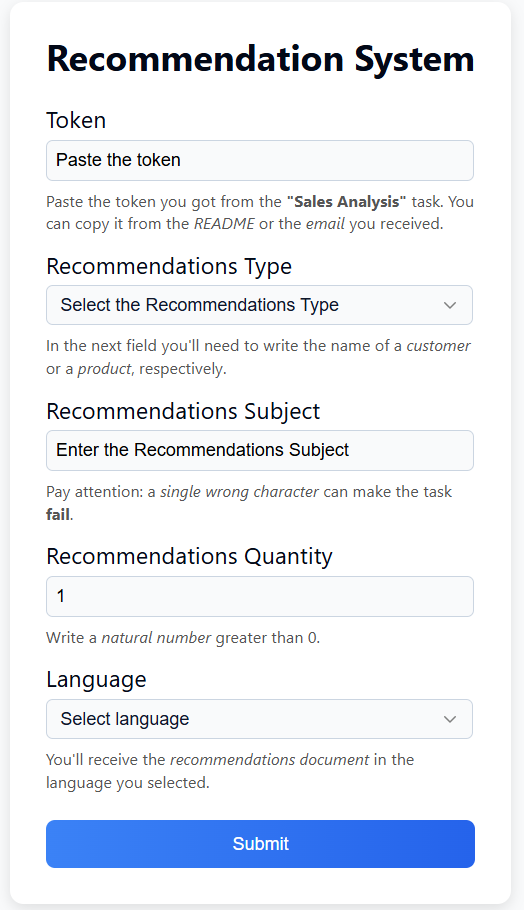
\includegraphics[width=\textwidth]{Frontend Recommendation.png}
			\end{minipage}
		\end{figure}
	\end{frame}


	\section{Ottimizzazione}

	\begin{frame}{Ottimizzazione}
		Nam libero tempore, cum soluta nobis est eligendi optio cumque nihil impedit quo minus id quod maxime placeat facere possimus.

		\begin{itemize}
			\item Ottimizzazione delle performance
			\item Riduzione dei costi computazionali
			\item Miglioramento dell'accuratezza
			\item Scalabilità del sistema
		\end{itemize}

		\begin{exampleblock}{Risultati}
			Omnis voluptas assumenda est, omnis dolor repellendus. Temporibus autem quibusdam et aut officiis debitis.
		\end{exampleblock}
	\end{frame}


	\section{Conclusioni e considerazioni finali}

	\begin{frame}{Conclusioni e considerazioni finali}
		Sed ut perspiciatis unde omnis iste natus error sit voluptatem accusantium doloremque laudantium, totam rem aperiam, eaque ipsa quae ab illo inventore veritatis et quasi architecto beatae vitae dicta sunt explicabo.

		\begin{block}{Risultati ottenuti}
			\begin{itemize}
				\item Miglioramento significativo delle performance del sistema
				\item Riduzione dei tempi di elaborazione
				\item Aumento dell'accuratezza delle raccomandazioni
				\item Scalabilità dimostrata in ambiente di produzione
			\end{itemize}
		\end{block}

		\begin{alertblock}{Sviluppi futuri}
			Nemo enim ipsam voluptatem quia voluptas sit aspernatur aut odit aut fugit, sed quia consequuntur magni dolores eos qui ratione voluptatem sequi nesciunt.
		\end{alertblock}
	\end{frame}

	\begin{frame}{Domande?}
		\begin{center}
			\Large
			\textbf{Grazie per l'attenzione!}
			
			\vspace{1em}
			
			\normalsize
			\textit{Presentazione disponibile su:}\\
			\url{https://github.com/username/presentazione-tesi}
			
			\vspace{2em}
			
			\Large
			\textbf{Ci sono domande?}
		\end{center}
	\end{frame}


\end{document}
